\documentclass[12pt, letterpaper]{report}
\usepackage[margin=1in]{geometry}
\usepackage[utf8]{inputenc}
\usepackage{graphicx}
\usepackage{float}
\usepackage{subfig}
\graphicspath{ {./img/} }
\setlength\parindent{0pt}
\renewcommand\thesection{\arabic{section}.}
\renewcommand{\thesubsection}{(\alph{subsection})}


\title{ECE1166 - MPI Analysis}
\author{Zachary M. Mattis}


\begin{document}
	
\maketitle


\section{MPI Point-to-Point (P2P) Communication}

MPI is a standardized method for spreading the execution of instructions among multiple processors to increase overall performance. Point-to-point communication is a method for sending data from one processor directly to another, much like sending a letter. MPI includes methods for determining the number of available processors, as well as which processor you are within the MPI environment. By doing so, a processor can effectively send and receive communications from a specified processor within its environment, as provided by the communication functions. Additionally, MPI providers support for stopping the executing process until it has received the necessary data to continue. This essential attribute is known as blocking, which allows these simultaneous processes to effectively interact with one another's data, ensuring that it is there before continuing. Through the addition of tags, processors can differentiate between messages from the same processors, a very important feature as there is no guarantee as to the order in which packets arrive.

\section{MPI Functions}

\begin{verbatim}
1. int MPI_Init( int *argc, char ***argv )
\end{verbatim}

MPI\_Init() is a function that is used by all MPI programs to initialize the execution environment, called at the beginning of the program.

\begin{verbatim}
2. int MPI_Finalize( void )
\end{verbatim}

MPI\_Finalize() is a function that is used by all MPI programs to terminate the execution environment, called at the end of the program.

\begin{verbatim}
3. int MPI_Comm_size( MPI_Comm comm, int *size )
\end{verbatim}

MPI\_Comm\_size determines the total number of available processors for a given MPI environment. This allows for dynamically scaling of a program dependent upon the total processing availability.

\begin{verbatim}
4. int MPI_Comm_rank( MPI_Comm comm, int *rank )
\end{verbatim}

MPI\_Comm\_rank is used by an MPI program to determine which processor it is the MPI environemnt. This allows for a single source code program to dynamically assign work to each individual processor.

\section{Distrubed Computing}

% A
\subsection{MPI\_Recv() Blocking}

A blocking function in computer programming is one in which the processor's execution is halted from continuing until an external I/O operation finishes its execution. In MPI\_Recv(), the processor will wait until it has received all of the data from the sender process until it continues with its own execution.

% B
\subsection{Parallel Efficiency}

Blocking reduces parallel efficiency because when a processor is in a state of blocking, it is unable to do any useful work because it is simply waiting for the data to be transferred by the communication function. Because a serial application does not need to communicate data among different processors, all of this communication is parallel overhead.

% C
\subsection{Application Blocking}

A web server is a great example of an application that spends the majority of its time waiting for network, filesystem, and database I/O operations to complete. In this architecture, the web server cannot continually process requests until all of its I/O operations have been completed for the previous request.

% D
\subsection{Blocking Alternatives}

This I/O bound system necessitates an application architecture that is highly scalable, allowing for the processing of multiple requests. This situation led  to the creation of Node.js, a non-blocking event loop based web server architecture that allows the web server to continually process requests while waiting for the I/O operations to finish in the background.

\section{Matrix Multiplication}

Given the data from the table below, both matrices of size 10 and 100 demonstrated an increase in execution time as the number of processors increased. This seems counter-intuitive on first look, but the parallel communication overhead must be taken into account to understand why more processors would actually result in a slowdown of execution time. However, one the matrix reaches a size of 1000, a decrease in the execution time can be observed, as the processing capabilities of more nodes offsets the parallel communication overhead, as previously mentioned. 

\begin{center}
	\begin{tabular}{ |l|l|l| } 
		\hline
		Matrix Size & Num Processors & Time (us) \\
		\hline
		10 & 2 & 55.789948 \\
		\hline
		10 & 4 & 102.043152 \\
		\hline
		10 & 8 & 119.924545 \\
		\hline
		10 & 16 & 199.079514 \\
		\hline
		100 & 2 & 725.030899 \\
		\hline
		100 & 4 & 864.028931 \\
		\hline
		1000 & 8 & 1572.847366 \\
		\hline
		1000 & 16 & 1702.070236 \\
		\hline
		1000 & 2 & 42989.96925 \\
		\hline
		1000 & 4 & 26597.97669 \\
		\hline
		1000 & 8 & 20676.13602 \\
		\hline
		1000 & 16 & 19587.99362 \\
		\hline
	\end{tabular}
\end{center}


\section{Ping-Pong}

The linear regression from the Ping-Pong test on Pitt's CRC cluster yielded approximate latency $\lambda\approx13 \mu s$ and bandwidth $\beta\approx870 bytes/\mu s$. Both the synchronous and asynchronous methods of communication provided very similar executions times of the Ping-Pong test, as illustrated in figures 1 and 2 below. From this data set, there is not statically difference in the communication times between synchronous vs. asynchronous MPI functions.

\begin{figure}[H]
	\captionsetup[subfigure]{labelformat=empty}
	\centering
	\subfloat[Figure 1]{{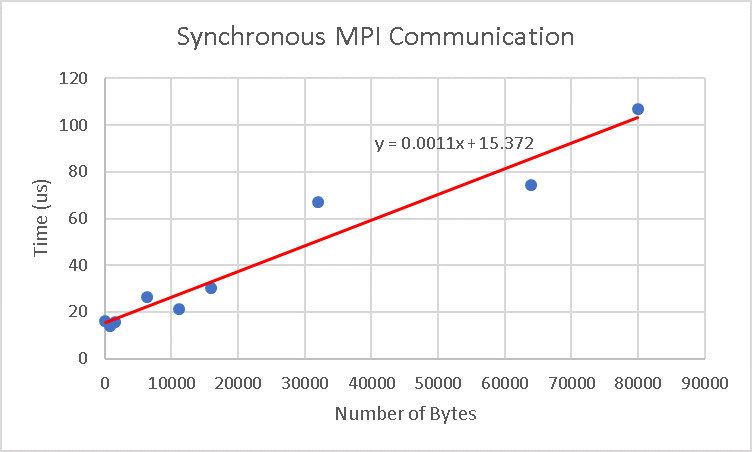
\includegraphics[width=18em]{sync.png} }}
	\qquad
	\subfloat[Figure 2]{{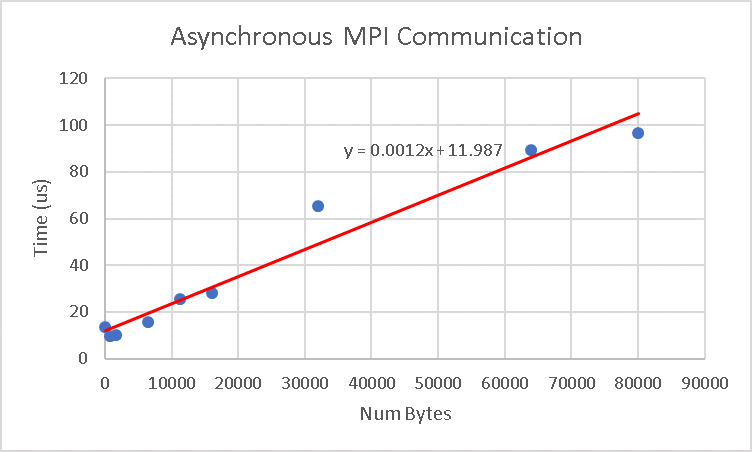
\includegraphics[width=18em]{async.png} }}
	\label{fig:example}
\end{figure}

Given my understanding of the different communication paradigms after completion of this project, I would implement each of them is a single ping\_ping.c file that would utilize a command line argument to determine the type of communication to use instead of each in a separate file. The current implementation was simpler as I was able to isolate each communication to a separate file.


\end{document}